\documentclass{beamer}
\usepackage{tikz}
\title{Algebra of Sequential Decision Problems}
\subtitle{formalised in Agda}
\author{Robert Krook \and \textbf{Patrik Jansson}}
\date{2020-01-06, WG2.1 \#79 in Otterlo, NL}
\begin{document}
\maketitle
\begin{abstract}
TODO
\end{abstract}

\begin{frame}
  \frametitle{Example: 1-dimensional coordinate system}

  \begin{tikzpicture}[
    arr/.style={thick, ->},
    ]
    \draw[arr] (0,0) -- coordinate (x axis mid) (6,0) node(xline)[right]{$\cdots$};
    % ticks
    \foreach \x in {0,...,5}
      \draw (\x,1pt) -- (\x,-3pt)
        node[anchor=north] {\x};
    \only<1>{\draw[arr] (0,1.5) -- (0,0.2) node[midway,right] {Right}; }
    \only<2>{\draw[arr] (1,1.5) -- (1,0.2) node[midway,right] {Right};}
    \only<3>{\draw[arr] (2,1.5) -- (2,0.2) node[midway,right] {Left};}
    \only<4>{\draw[arr] (1,1.5) -- (1,0.2) node[midway,right] {Stay};}
  \end{tikzpicture}

\end{frame}
\end{document}

\begin{tikzpicture}[y=.2cm, x=.7cm,font=\sffamily]
 	%axis
	\draw (0,0) -- coordinate (x axis mid) (10,0);
    	\draw (0,0) -- coordinate (y axis mid) (0,30);
    	%ticks
    	\foreach \x in {0,...,10}
     		\draw (\x,1pt) -- (\x,-3pt)
			node[anchor=north] {\x};
    	\foreach \y in {0,5,...,30}
     		\draw (1pt,\y) -- (-3pt,\y)
     			node[anchor=east] {\y};
	%labels
	\node[below=0.8cm] at (x axis mid) {MOPS};
	\node[rotate=90, above=0.8cm] at (y axis mid) {Power [mW]};

	%plots
	\draw plot[mark=*, mark options={fill=white}]
		file {div_soft.data};
	\draw plot[mark=triangle*, mark options={fill=white} ]
		file {div_ciu.data};
	\draw plot[mark=square*, mark options={fill=white}]
		file {div_ciu_oscar.data};
	\draw plot[mark=square*]
		file {div_ciu_oscar_extrapolated.data};

	%legend
	\begin{scope}[shift={(4,4)}]
	\draw (0,0) --
		plot[mark=*, mark options={fill=white}] (0.25,0) -- (0.5,0)
		node[right]{soft};
	\draw[yshift=\baselineskip] (0,0) --
		plot[mark=triangle*, mark options={fill=white}] (0.25,0) -- (0.5,0)
		node[right]{ciu};
	\draw[yshift=2\baselineskip] (0,0) --
		plot[mark=square*, mark options={fill=white}] (0.25,0) -- (0.5,0)
		node[right]{ciu + oscar};
	\draw[yshift=3\baselineskip] (0,0) --
		plot[mark=square*, mark options={fill=black}] (0.25,0) -- (0.5,0)
		node[right]{ciu + oscar extrapolated};
	\end{scope}
\end{tikzpicture}

% ----------------------------------------------------------------
\usetikzlibrary{arrows}
% ..
\begin{tikzpicture}[
    scale=5,
    axis/.style={very thick, ->, >=stealth'},
    important line/.style={thick},
    dashed line/.style={dashed, thin},
    pile/.style={thick, ->, >=stealth', shorten <=2pt, shorten
    >=2pt},
    every node/.style={color=black}
    ]
    % axis
    \draw[axis] (-0.1,0)  -- (1.1,0) node(xline)[right]
        {$G\uparrow/T\downarrow$};
    \draw[axis] (0,-0.1) -- (0,1.1) node(yline)[above] {$E$};
    % Lines
    \draw[important line] (.15,.15) coordinate (A) -- (.85,.85)
        coordinate (B) node[right, text width=5em] {$Y^O$};
    \draw[important line] (.15,.85) coordinate (C) -- (.85,.15)
        coordinate (D) node[right, text width=5em] {$\mathit{NX}=x$};
    % Intersection of lines
    \fill[red] (intersection cs:
       first line={(A) -- (B)},
       second line={(C) -- (D)}) coordinate (E) circle (.4pt)
       node[above,] {$A$};
    % The E point is placed more or less randomly
    \fill[red]  (E) +(-.075cm,-.2cm) coordinate (out) circle (.4pt)
        node[below left] {$B$};
    % Line connecting out and ext balances
    \draw [pile] (out) -- (intersection of A--B and out--[shift={(0:1pt)}]out)
        coordinate (extbal);
    \fill[red] (extbal) circle (.4pt) node[above] {$C$};
    % line connecting  out and int balances
    \draw [pile] (out) -- (intersection of C--D and out--[shift={(0:1pt)}]out)
        coordinate (intbal);
    \fill[red] (intbal) circle (.4pt) node[above] {$D$};
    % line between out og all balanced out :)
    \draw[pile] (out) -- (E);
\end{tikzpicture}
%%% Local Variables:
%%% mode: latex
%%% TeX-master: t
%%% End: